\section{Team}

\subsection*{Feature Descriptors (SIFT)}

This section details the front-end implementation of a visual odometry system based on feature matching. The core task is to create stable correspondences between successive image frames by identifying and comparing unique visual landmarks. We chose the \emph{Scale-Invariant Feature Transform (SIFT)} for its strong performance under varying scales and rotations. The code is designed to isolate the feature extraction algorithm from the broader tracking workflow, making it straightforward to swap in different methods later.

This file \lstinline{sift\_feature\_tracker.cpp} \ref{sub:sift_feature_tracker_cpp} contains the core implementation of the SIFT algorithm.

The \lstinline{detectKeypoints} and \lstinline{describeKeypoints} functions rely on OpenCV's \lstinline{SIFT::create()}. SIFT finds keypoints by locating peaks in the Difference of Gaussians (DoG) pyramid across different scales, which gives it scale invariance. It then builds a 128-element descriptor vector from the distribution of gradient directions around each keypoint, providing rotation invariance.

In file \lstinline{feature\_tracker.cpp}, we updated the \lstinline{trackFeatures} function to manage the processing steps. It calls \lstinline{detectKeypoints} on both images. Running the command \lstinline{roslaunch lab\_5 two\_frames\_tracking.launch descriptor:=SIFT} generates a visualization of the matched features.

The figures~\ref{fig:local_feature_extraction_sift_keypoints_} show the results. Keypoints, drawn with their detected size and orientation, cluster in textured regions like the printed text and box edges. This demonstrates the detector's ability to find distinctive image patterns.

\begin{figure}[htb]
  \centering
  \begin{subfigure}{0.8\linewidth}
    \includegraphics[width=\linewidth]{figures/sift_keypoints_1}
  \end{subfigure}
  \hfill
  \begin{subfigure}{0.8\linewidth}
    \includegraphics[width=\linewidth]{figures/sift_keypoints_2}
  \end{subfigure}
  \caption{Local Feature Extraction (SIFT Keypoints)}
  \label{fig:local_feature_extraction_sift_keypoints_}
\end{figure}

\subsection*{Feature Matching via Descriptors}

This part connects the features found earlier by matching them across images. We built the \lstinline{matchDescriptors} function in \lstinline{sift\_feature\_tracker.cpp} to handle this.

Rather than using a slow, exhaustive search, we chose a \emph{FLANN-based matcher} with a K-Nearest Neighbors approach (KNN, \(k=2\). To weed out unreliable matches, we added \emph{Lowe's Ratio Test} as a filter.

The test works by checking:

\begin{equation*}
d_1 < \text{ratio} \cdot d_2
\end{equation*}

Here, \(d_1\) is the distance to the best-matching descriptor, and \(d_2\) is the distance to the second-best. We kept the ratio threshold at \(0.8\). This helps ignore ambiguous matches—like those from the box's repeating patterns—and tightens up the overall match quality.

You can see the results~\ref{fig:feature_matching_results_after_ratio_test_filtering_}. While most matches correctly pair up similar parts of the box (corners with corners, for example), some \emph{outliers} still slip through (shown by crossing lines). These mismatches break the expected smooth motion between frames, showing that matching based on looks alone isn't enough.

\begin{figure}[htb]
  \centering
  \includegraphics[width=0.8\linewidth]{figures/sift_matches}
  \caption{Feature Matching Results (After Ratio Test Filtering)}
  \label{fig:feature_matching_results_after_ratio_test_filtering_}
\end{figure}

\subsection*{Matching Quality Refinement}

To clean up the remaining bad matches, we added Geometric Verification in \lstinline{feature\_tracker.cpp} through the \lstinline{inlierMaskComputation} function.

The method uses \emph{RANSAC (Random Sample Consensus)} to find the best Fundamental Matrix (\(F\) that fits the matched points. The core idea is the \emph{Epipolar Constraint}:

\begin{equation*}
p_2^\top F p_1 = 0
\end{equation*}

Here, \(p_1\) and \(p_2\) are matched points in the first and second images (in homogeneous coordinates). Matches that don't follow this rule within \(3.0\) pixels are thrown out as outliers.

\begin{figure}[htb]
  \centering
  \includegraphics[width=0.8\linewidth]{figures/sift_inliers}
  \caption{Inliers after RANSAC verification}
  \label{fig:inliers_after_ransac_verification}
\end{figure}

Compared to the results from Deliverable 4, \ref{fig:inliers_after_ransac_verification} the crossing mismatch lines are now gone. The surviving matches (inliers) show a clean, consistent motion pattern, which better reflects the actual camera movement around the box.

The terminal output looked like:
\begin{minted}{text}
Avg. Keypoints 1 Size: 603
Avg. Keypoints 2 Size: 969
Avg. Number of matches: 603
Avg. Number of good matches: 98
Avg. Number of Inliers: 77
Avg. Inliers ratio: 0.785714
Num. of samples: 1
\end{minted}

\subsection*{Comparing Feature Matching Algorithms on Real Data}

This section tests three more feature matching algorithms alongside SIFT: \emph{SURF}, \emph{ORB}, and \emph{FAST+BRIEF}. We want to see how they stack up against our SIFT baseline in different situations.

We wrote C++ classes for each method (\lstinline{SurfFeatureTracker}, \lstinline{OrbFeatureTracker}, \lstinline{FastFeatureTracker}). One important note: matching works differently for floating-point descriptors (SIFT/SURF) and binary ones (ORB/BRIEF). For SIFT/SURF we use Euclidean distance, but for ORB/BRIEF we switch to Hamming distance, which is faster and more appropriate for binary data.

We ran tests in two scenarios: Pair of Frames, where two images with a big viewpoint change (rotation and scale), and Real Datasets (Video), where continuous video to see how they handle small, sequential motions.

\subsubsection*{Pair of Frames}

\begin{figure}[!htb]
  \centering
  \includegraphics[width=0.8\linewidth]{figures/demonstration_frame}
  \caption{Demo: processing two frames}
  \label{fig:demo_processing_two_frames}
\end{figure}

We ran this command four times, once for each method (SIFT, SURF, ORB, FAST+BRIEF):

\begin{minted}{console}
roslaunch lab_5 two_frames_tracking.launch descriptor:=<METHOD>
\end{minted}

The terminal outputs were in the appendix~\ref{ssub:a_pair_of_frames}. From these logs, we analyse and compare the \emph{floating-point} and the \emph{binary} methods:

\begin{enumerate}
  \item Floating-point methods (SIFT/SURF): Both did well with the big viewpoint change. SIFT had a solid 78.6\% inlier ratio. SURF found more keypoints but was a bit less accurate (66.7\%).
  \item Binary methods (ORB/FAST+BRIEF): These struggled more with the large baseline. \emph{FAST+BRIEF} found tons of keypoints but had a low inlier rate (41.5\%). BRIEF isn't built for big rotations, which explains it. At the same time, \emph{ORB} gave very few good matches (only 8), likely because Lowe's Ratio Test was too strict with Hamming distance on this texture. But the matches that passed were very accurate (87.5\% inliers).
\end{enumerate}

\subsubsection*{Real Datasets}

Next, we tested on two video datasets with this command (run for each method):

\begin{minted}{console}
roslaunch lab_5 video_tracking.launch path_to_dataset:=/home/$USER/Desktop/<DATASET>.bag descriptor:=<METHOD>
\end{minted}

\textbf{\lstinline{30fps_424x240_2018-10-01-18-35-06.bag}}

\begin{figure}[!htb]
  \centering
  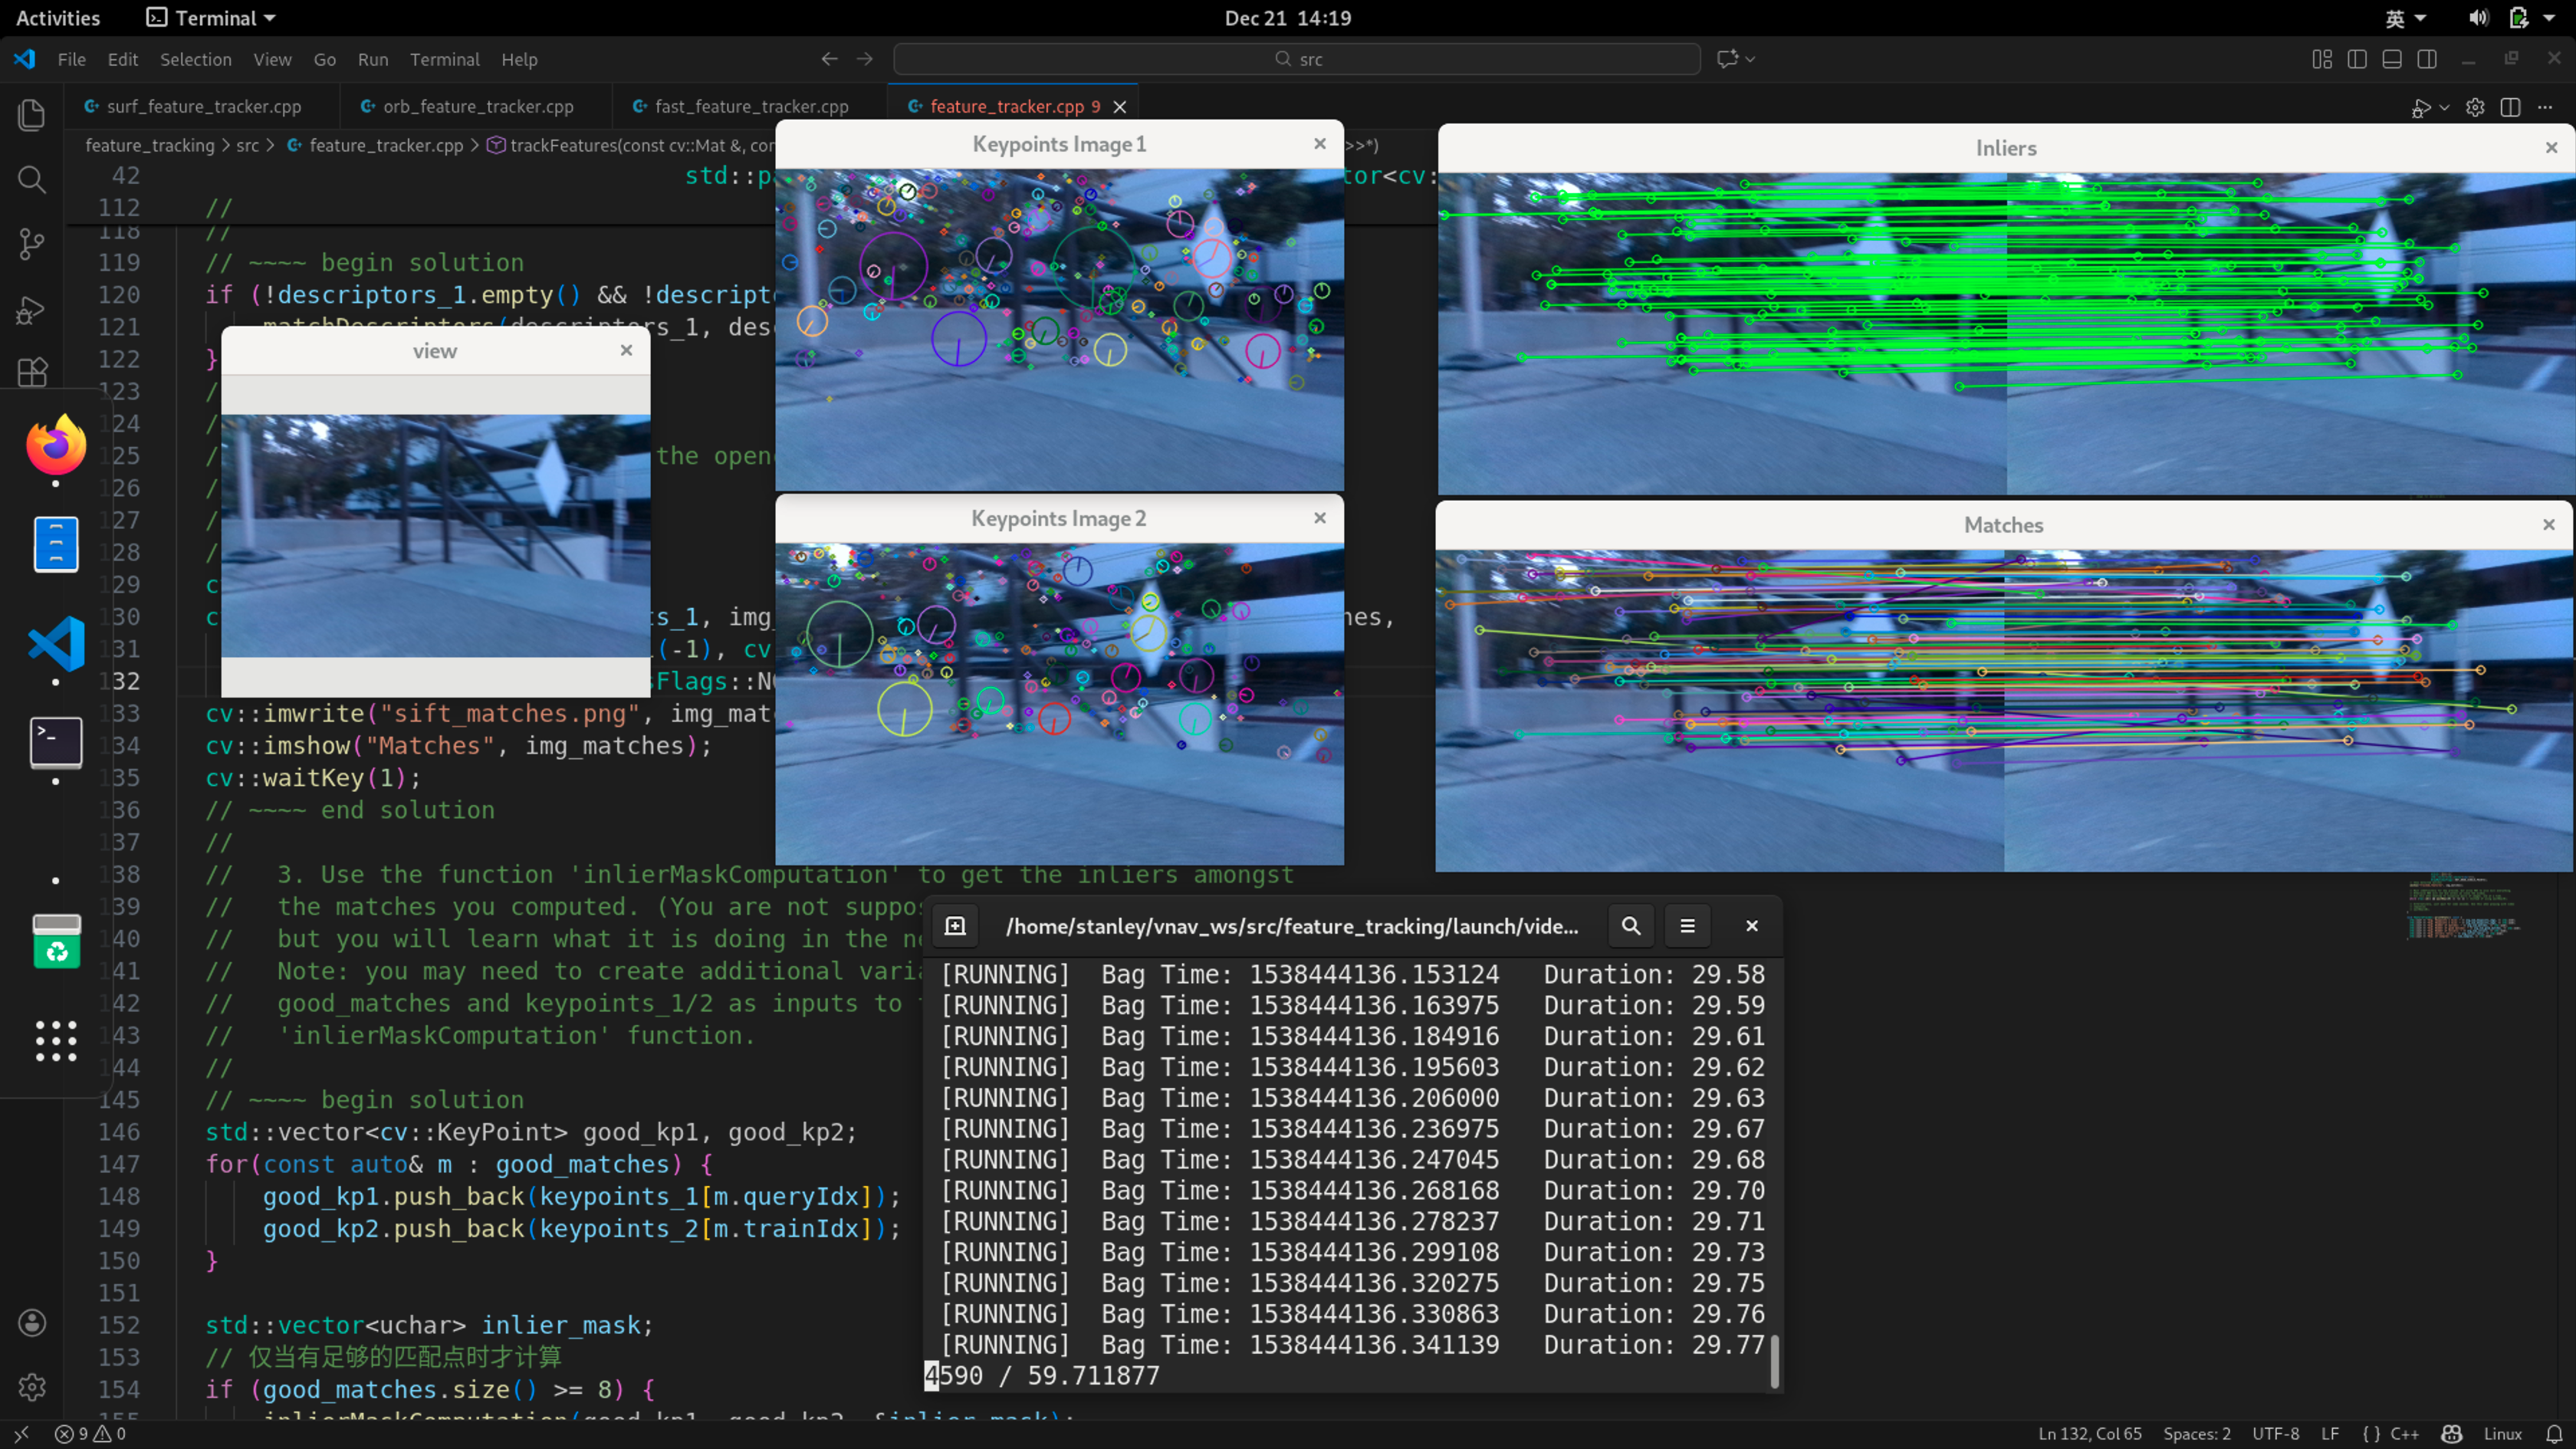
\includegraphics[width=0.8\linewidth]{figures/demonstration_video_30fps}
  \caption{Processing the 30fps video}
  \label{fig:processing_the_30fps_video}
\end{figure}

And the logs are in appendix~\ref{ssub:a_real_datasets}. Through whose data, we found out two results for Video Sequences. Binary methods are more precise here. In continuous video, ORB and FAST+BRIEF had higher inlier ratios (88\%) than SIFT/SURF (75-78\%). For small, sequential motions, binary descriptors gave cleaner matches. Feature density varies a lot. SURF found the most features (over 1000 per frame) and kept the most inliers (345), giving a dense tracking field. This is good for robustness but slow. While SIFT was sparse (~50 inliers), which could be risky if the scene lacks texture, FAST+BRIEF struck a balance: good density (273 inliers) with high accuracy. Speed differences were obvious. ORB and FAST+BRIEF ran fast, suitable for real-time use. SURF felt slow because it processes so many floating-point descriptors per frame.

This came out a conclusion. For tasks with big viewpoint changes (like loop closure), use \emph{SIFT} or \emph{SURF}, while for real-time visual odometry with small motions, \emph{ORB} or \emph{FAST+BRIEF} gives the best speed/accuracy trade-off.

\subsection*{Lucas Kanade Feature Tracking}

This final part implements the Lucas-Kanade (LK) tracker, which works differently from the descriptor-based methods (SIFT, SURF, ORB) we tested earlier.

Instead of finding and matching features between frames, LK tracks them using the \emph{Brightness Constancy Assumption}:

\begin{equation*}
I(x, y, t) \approx I(x+d x, y+d y, t+d t)
\end{equation*}

It calculates the motion vector \((u, v)\) by minimizing the error in a small window, using image gradients. We used OpenCV's \lstinline{cv::calcOpticalFlowPyrLK} with an image pyramid to handle larger movements. Tracking starts with \emph{Good Features to Track (GFTT)} in the first frame.

We ran the LK tracker on the same two real-world datasets. The code is in appendix~\ref{sub:lk_feature_tracker_cpp} and the results are in Fig.~\ref{fig:lucas_kanade_tracking_results_on_real_datasets}.

\begin{figure}[tb]
  \centering
  \begin{subfigure}{0.8\linewidth}
    \includegraphics[width=\linewidth]{figures/LK_30fps}
  \end{subfigure}
  \hfill
  \begin{subfigure}{0.8\linewidth}
    \includegraphics[width=\linewidth]{figures/LK_vnav}
  \end{subfigure}
  \caption{Lucas Kanade tracking results on real datasets}
  \label{fig:lucas_kanade_tracking_results_on_real_datasets}
\end{figure}

\textbf{Dataset: \lstinline{30fps_424x240_2018-10-01-18-35-06.bag}}

\begin{minted}{text}
[INFO] [1766307648.340722934]: LK Stats: Matches: 776 Inliers: 756 Ratio: 0.974227
\end{minted}

\textbf{Dataset: \lstinline{vnav-lab5-smooth-trajectory.bag}}

\begin{minted}{text}
[INFO] [1766308353.398518896]: LK Stats: Matches: 653 Inliers: 634 Ratio: 0.970904
\end{minted}

\emph{What we observed that the highest inlier ratio is over 97\%, LK had the cleanest matches (97.4\% inliers). Descriptor matching (like SIFT/ORB) searches globally, so a feature in one corner might match a similar-looking feature in the opposite corner (an outlier). LK only searches locally, assuming features don't move far between frames. This naturally avoids those big mistakes in smooth videos. We didn't log exact timings, but LK is faster because it skips computing descriptors and doing brute-force matching. It just uses image gradients, which is great for real-time needs (like drone control). LK worked so well here because our videos had smooth, small motions (30fps). If the camera moved too fast or frames were skipped, LK would lose track. Descriptor-based methods like SIFT/ORB are better at handling big jumps.}

Lucas-Kanade gives the most accurate and efficient tracking for \emph{smooth, continuous video}. But it can't re-lost features or match across big viewpoint changes—for that, you still need descriptor-based methods like ORB or SIFT.

\subsection*{Optical Flow}

\begin{figure}[!htb]
  \centering
  \begin{subfigure}{0.8\linewidth}
    \includegraphics[width=\linewidth]{figures/farneback_30fps}
  \end{subfigure}
  \hfill
  \begin{subfigure}{0.8\linewidth}
    \includegraphics[width=\linewidth]{figures/farneback_vnav}
  \end{subfigure}
  \caption{Dense Optical Flow using Farneback's method}
  \label{fig:dense_optical_flow_using_farneback_s_method}
\end{figure}

The Farneback algorithm estimates optical flow for \emph{every pixel} in the image, unlike the sparse methods (SIFT/LK) we tested before. You can see our implementation~\ref{sub:self_flow_cpp}. In the figures above, we visualize the flow field in HSV colors: \emph{Hue} indicates direction of motion, and \emph{Value} shows how fast the pixel is moving.

The LK tracker is efficient for following specific points, which works well for tasks like SLAM. Farneback gives a motion vector at each pixel, which paints a fuller picture of how everything in the scene is moving—you can even make out the shape of the box from the flow. The downside is speed: calculating flow everywhere is heavy, and we noticed a clear slowdown compared to the real-time LK tracker.
